\documentclass{cshwk}

\begin{document}

\title{HW \#2, Chapter 2}

\maketitle

\section*{Problem 4. Chapter 2 P22.}


Consider distributing a file of \( F = 20 \) Gbits to \( N \) peers. The server has an upload rate of \( u_s = 30 \) Mbps, and each peer has a download rate of \( d_i = 2 \) Mbps and an upload rate of \( u \). For \( N = 10, 100, \) and \( 1,000 \) and \( u = 300 \) Kbps, 700 Kbps, and 2 Mbps, prepare a chart giving the minimum distribution time for each of the combinations of \( N \) and \( u \) for both client-server distribution and P2P distribution.

\subsection*{Solution}



\subsubsection*{Client-Server Distribution}

\begin{figure}[H]
    \centering
    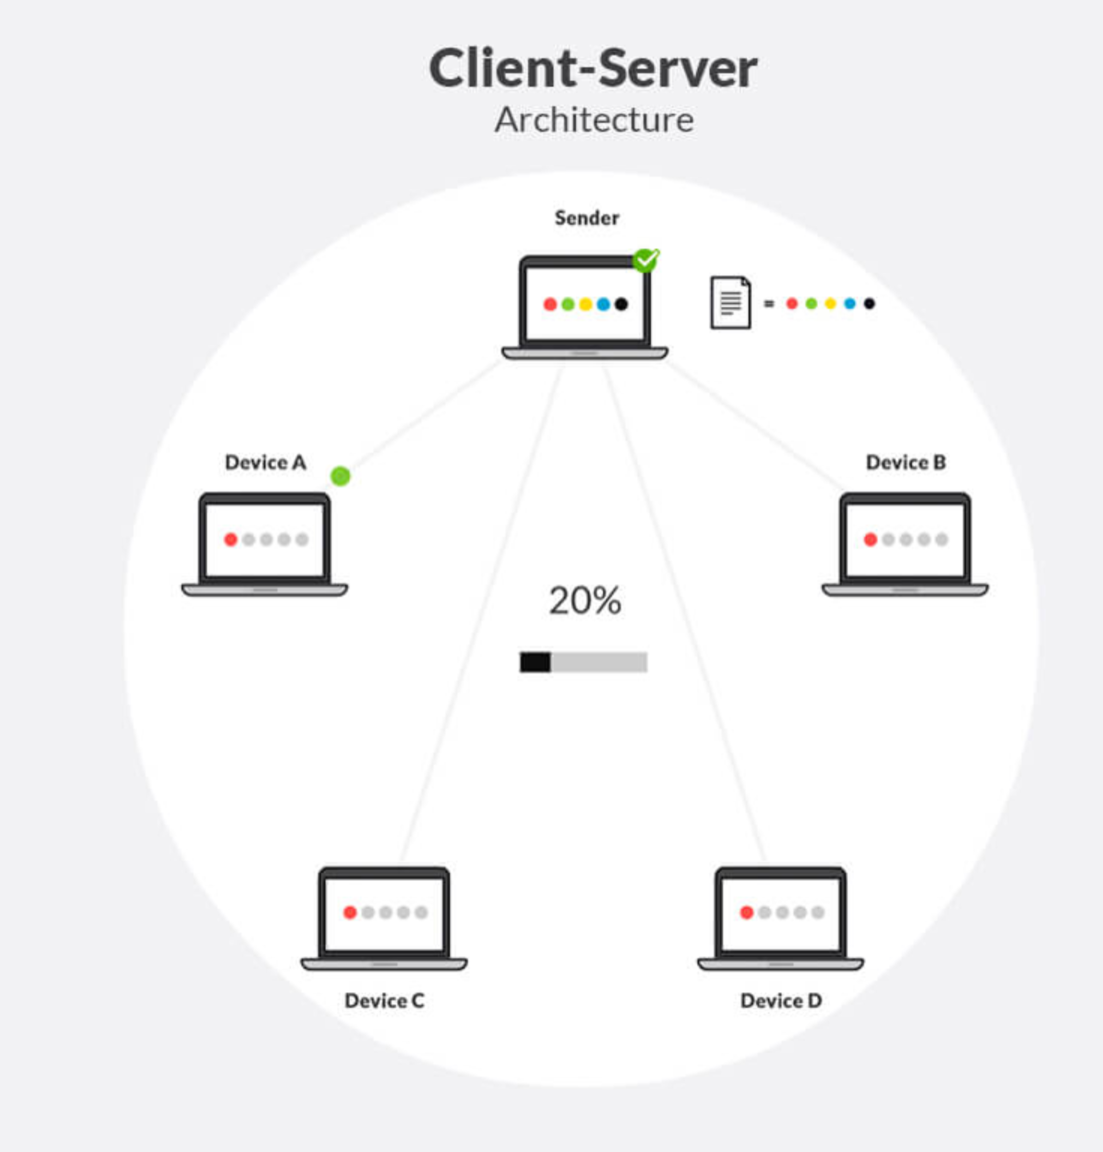
\includegraphics[width=0.4\textwidth]{hw2-4-1.png}
    \caption{Client-Server Model}
    \label{fig:cs}
\end{figure}
In \texttt{Client-Server} Distribution model, the file is send from the server to each client individually. the bottleneck link is the server's upload link or the peer's download speed. The server needs to upload the file to each client. Therefore, the minimum distribution time is given by:

\begin{equation*}
    t_{cs} =
    \begin{cases}
        \frac{F}{u_s / N} & \text{if } N \times d_i \geq u_s (\text{upload link bottleneck}) \\
        \frac{F}{d_i}     & \text{if } N \times d_i < u_s (\text{download link bottleneck})
    \end{cases}
\end{equation*}

Therefore, the distribution time for the \texttt{Client-Server} model is inralevant to the upload speed of the peers. The distribution time is given in the Tab.~\ref{tab:cs}.

\begin{table}[H]
    \centering
    \begin{tabular}{cc}
        \toprule
        \( N \) & \( t_{cs} \)                                                \\
        \midrule
        10      & $\frac{F}{d_i} = \frac{20Gbits}{2Mbps} = 10,000s$           \\
        100     & $\frac{F}{u_s/N} = \frac{20Gbits}{30Mbps / 100} =66,667s $  \\
        1,000   & $\frac{F}{u_s/N} = \frac{20Gbits}{30Mbps/ 1000} = 666,667s$ \\
        \bottomrule
    \end{tabular}
    \caption{Client-Server Distribution Time}
    \label{tab:cs}
\end{table}

\subsubsection*{P2P Distribution}

\begin{figure}[H]
    \centering
    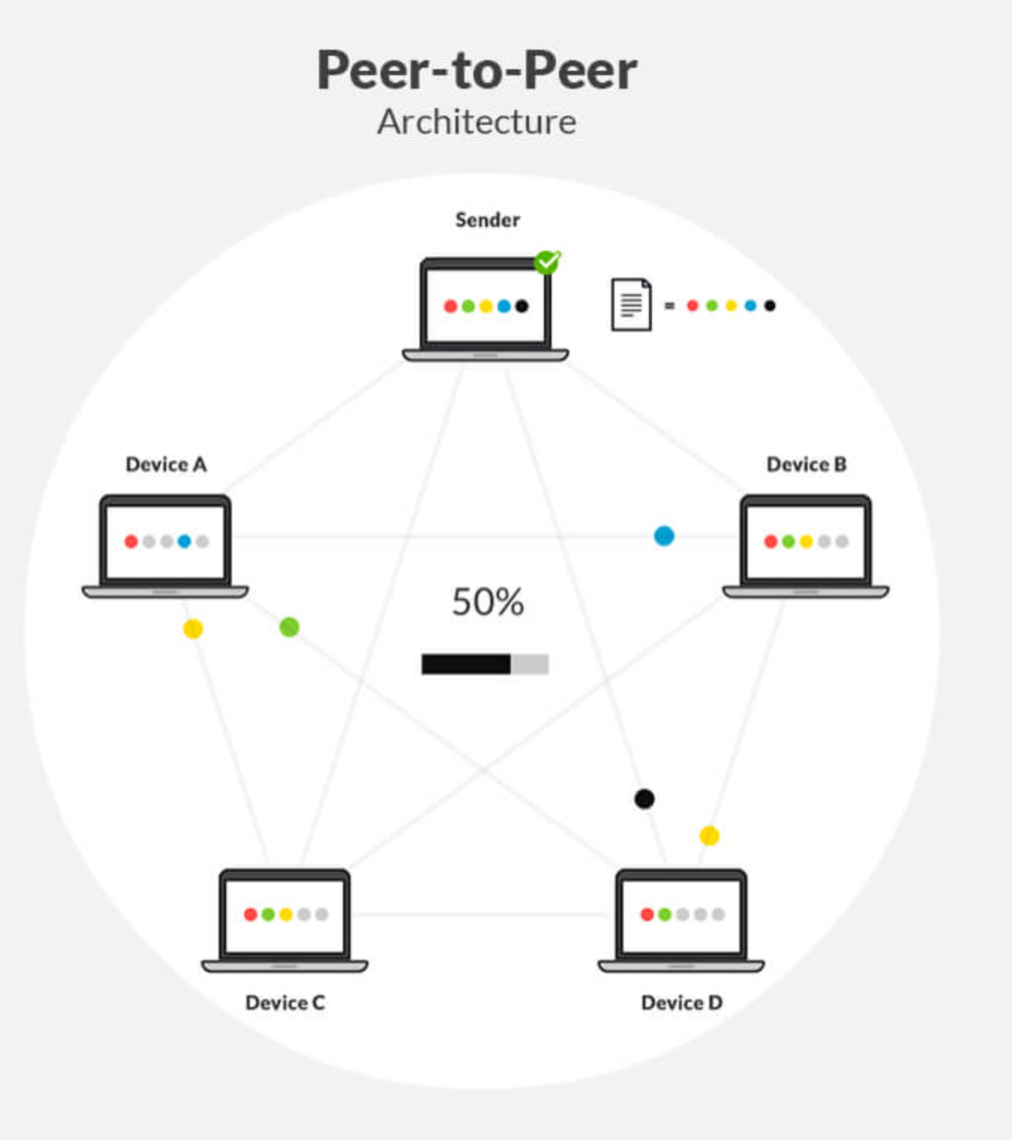
\includegraphics[width=0.4\textwidth]{hw2-4-2.png}
    \caption{P2P Model}
    \label{fig:p2p}
\end{figure}

In \texttt{P2P} Distribution model, the file is send from the server to the p2p networks. and then the peers share the file with each other. There are three cases for the bottleneck link:

\paragraph*{Case 1:} The server's upload link is the bottleneck link. In this case, the server needs to upload the file to all peers. The minimum distribution time is given by:

\begin{equation*}
    t_{upload} = \frac{F}{u_s}
\end{equation*}

\paragraph*{Case 2:} The peer's download link is the bottleneck link. In this case, the server needs to upload the file to only one peer. The minimum distribution time is given by:

\begin{equation*}
    t_{download} = \frac{F}{d_i}
\end{equation*}

\paragraph*{Case 3:} In this P2P network, a total of $N\times F$ bits of data is delivered across the network, which includes one server and all peer nodes. The total delivery time can be expressed as:

\begin{equation*}
    t_{sharing} = \frac{N\times F}{u_s + \sum_{i=1}^{N} u_i}
\end{equation*}

Therefore, the distribution time for the \texttt{P2P} model is given by:

\begin{equation*}
    t_{p2p} = \max \left( t_{upload}, t_{download}, t_{sharing} \right)
\end{equation*}

The distribution time is given in the Tab.~\ref{tab:p2p}.
\begin{table}[H]
    \centering
    \begin{tabular}{|c|c|c|c|}
        \hline
        \diagbox{N}{u} & 0.3 Mbps & 0.7 Mbps & 2 Mbps  \\
        \hline
        10             & 10000 s  & 10000 s  & 10000 s \\
        100            & 33333 s  & 20000 s  & 10000 s \\
        1000           & 60606 s  & 27397 s  & 10000 s \\   
        \hline
    \end{tabular}
    \caption{P2P Distribution Times with Different \( N \) and \( u \)}
    \label{tab:p2p}
\end{table}


\subsubsection*{Summary}

The distribution time can be shown in the Fig.~\ref{fig:summary}.
\begin{figure}[H]
    \centering
    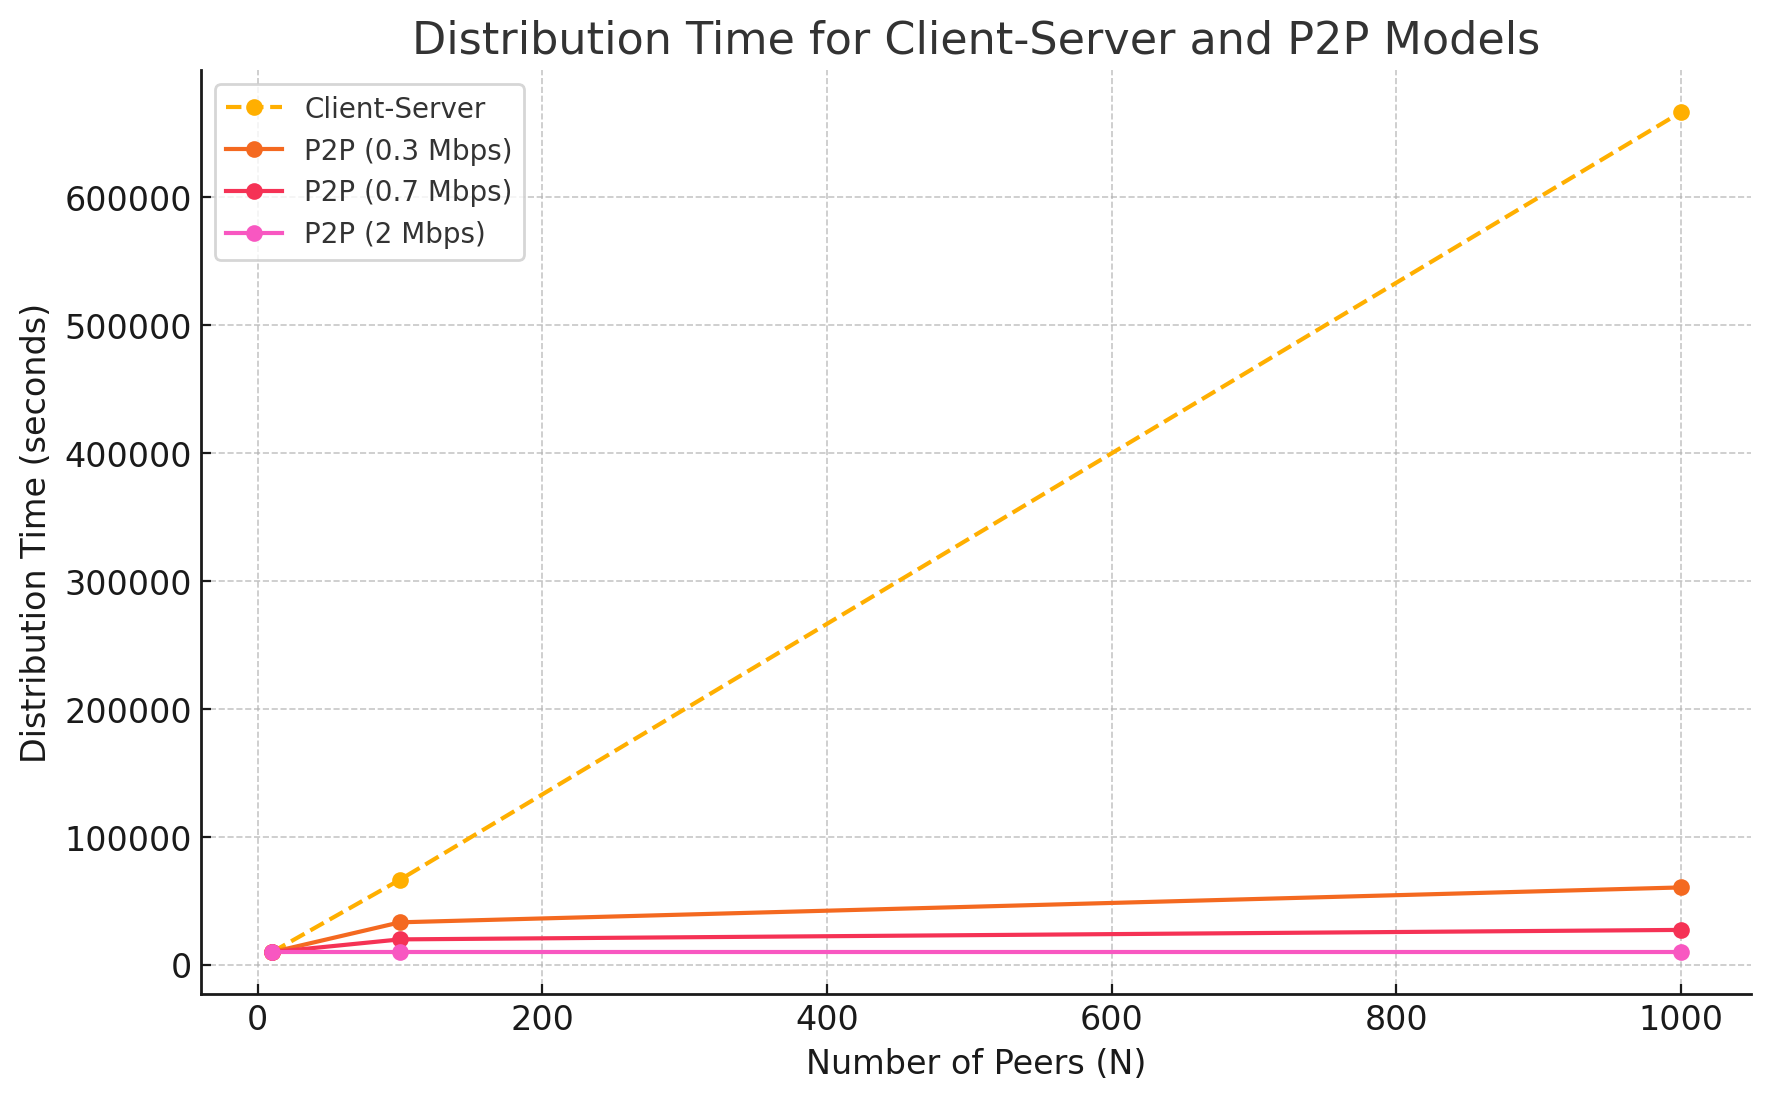
\includegraphics[width=0.6\textwidth]{hw2-4-3.png}
    \caption{Summary of Distribution Times}
    \label{fig:summary}
\end{figure}

From the Fig.~\ref{fig:summary}, we can see that the distribution time for the \texttt{Client-Server} model is irrelevant to the upload speed of the peers. However, the distribution time for the \texttt{P2P} model is relevant to the upload speed of the peers. The distribution time for the \texttt{P2P} model is shorter than the \texttt{Client-Server} model when the upload speed of the peers is larger than the server's upload speed.


\end{document}